\subsection{Implementación de hardware}
\subsubsection{Medición de estado de los SIS}

El SAL/T debe interactuar con 5 sistemas instrumentados de seguridad (SIS) que cada uno cuenta con 2 llaves de estado; una para la línea de la señal crítica de corte de tracción (CT) y la otra para la señal crítica de freno de emergencia (FE). Estas llaves van a estar en un estado cerrado cuando el SIS esté funcionando correctamente y no detecte ninguna situación peligrosa en la formación, y se van a abrir para interrumpir la alimentación de las señales críticas ante una falla en el SIS o la detección de alguna condición peligrosa. \\ 

Considerando el diagrama de conexión ya presentado en la figura \ref{fig:señales_criticas}, se puede interpretar que, cuando la llave está cerrada, por definición, la diferencia de tensión entre sus terminales va a ser nula. En cambio, si en toda la línea existe un único interruptor abierto, se espera que toda la tensión de alimentación $V_{ALIM}$ que en el terminal positivo de la llave mientras que en el terminal negativo, debería haber una tensión de tierra, ya que, al abrir el circuito, no va a circular corriente por la línea y la electroválvula no va a agregar ninguna caída de tensión. Por lo tanto, se pueden resumir la diferencia de tensión esperada en los terminales de un SIS en la tabla \ref{tab:switch_state}. 

\begin{table}[htb]
    \begin{tabular}{|c|c|} 
        \hline
        \textbf{Estado de llave} & \textbf{Tensión entre terminales}\\
        \hline
        Cerrada     &     0 V   \\
        \hline
        Abierta     &     $V_{ALIM}$ \\
        \hline
    \end{tabular}
    \label{tab:switch_state}
    \caption{Diferencia de tensión entre los terminales de un SIS}
\end{table}

Los rangos de tensión de alimentación de las baterías de las formaciones consideradas son $ 72 VDC < V_{ALIM} < 110 VDC $. Y considerando que estos buses de mayor tensión pueden no tener una puesta de tensión en común con el SAL/T, se decidió utilizar un circuito de medición diferencial para calcular la tensión entre las terminales de un interruptor independientemente de su tensión contra la tierra del circuito y luego conectar la tensión medida en un conversor analógico digital (ADC) del microcontrolador para poder obtener de manera digital un valor para la tensión. \\ 


Con el objetivo de alterar lo menos posible línea de las señales críticas, se optó por utilizar un amplificador de instrumentación para poder medir la tensión diferencial entre los terminales de las llaves. Este dispositivo permite medir una tensión diferencial rechazando cualquier señal de modo común con una gran impedancia de entrada lo que permite derivar una pequeña corriente de la línea principal sin alterarla. El modelo seleccionado fue el INA823DGKR de Texas Instrument \cite{INA823DGKR}; un amplificador de instrumentación con salide \textit{single-ended} con un rango de ganancia programable de 1 a 1000 con una resistencia externa, con una baja corriente de polarización de entrada de 1.2 nA y permite la alimentación con una fuente dual de $\pm1.1 V$ a $\pm18 V$. Para la aplicación en el SAL/T, se va a utilizar una ganancia de 1 (sin resistencia externa conectada) y se va a alimentar el amplificador con una tensión dual de $\pm5 V$.\\

Para generar la tensión de -5V a partir de la fuente de alimentación de +5V, se utilizó el regulador de tensión ICL7660AIBAZA de Renesas Electronics \cite{ICL7660AIBAZA} diseñado para invertir una tensión de entrada positiva y generar una salida negativa. Este permite la inversión de la tensión de entrada en el rango de 1.5 V a 12 V, tiene un bajo consumo de corriente de 80 $\mu$A, funciona con un oscilador interno a 10KHz que elimina la necesidad de generar una señal de reloj externa y solo requiere dos capacitores externos. El circuito integrado (CI) viene en un encapsulado VSSOP-8 para montaje superficial. En la figura \ref{fig:ICL7660AIBAZA}, se observa la conexión del ICL7660AIBAZA siguiendo las recomendaciones de la hoja de datos para una tensión de entrada de +5V; se utilizaron 2 capacitores electrolíticos de 10 $\mu$F y se obtuvo una tensión de salida de -5V. 

 
\begin{figure}[H]
    \centering
    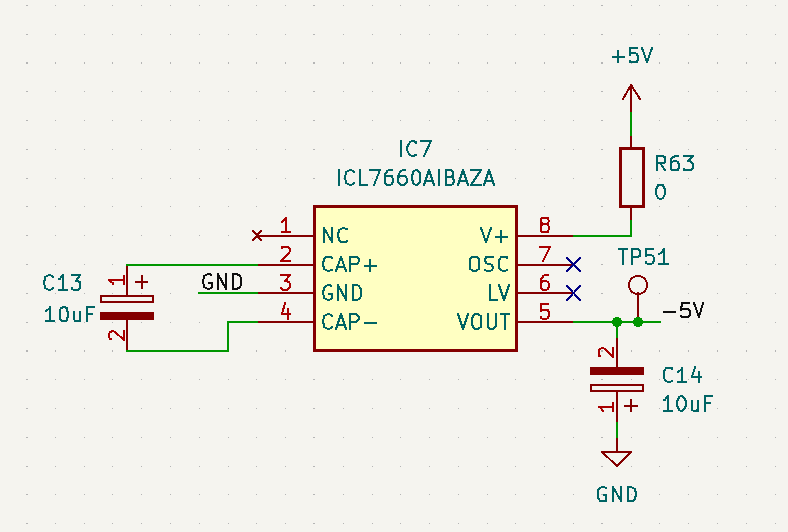
\includegraphics[width = 0.8 \linewidth]{img/ICL7660AIBAZA.png}
    \caption{Esquemático del circuito para generación de tensión de alimentación negativa}
    \label{fig:ICL7660AIBAZA}
\end{figure}


Para poder medir la tensión diferencial en las terminales de las llaves del SIS con el INA823DGKR alimentado con $\pm$5V, es necesario adaptar las tensiones a medir a un rango dentro de los extremos de la alimentación, ya que podría haber una diferencia de hasta 110V sobre esa llave. Para reducir esta tensión diferencial, se implementó una red de resistencias que permitan mantener la diferencia de tensión, pero reducida por un factor seleccionado y utilizando una tierra como referencia para tener las tensiones positivas y negativas a la entrada del amplificador de instrumentación. \\ 

Si bien el rango máximo para las entradas podía ser $\pm$5V, considerando que la ganancia del amplificador es 1 y que la salida va a ingresar a un ADC del microcontrolador que trabaja en un rango de hasta 3V3 de entrada, hay que reducir el rango máximo esperado hasta esa tensión. Por lo tanto, si consideramos 110 V como la máxima tensión diferencial en la llave del SIS, y armando una red de resistencias que parta esta tensión a la mitad colocando una tierra en la mitad del circuito, se debe calcular los valores de las resistencias tal que, en cada entrada del amplificador, haya como máximo una tensión de $\pm$1.65 V, ya que, la salida es \textit{single-ended} y para esos valores máximos usaría el rango completo de 3V3 del ADC. Considerando un divisor resistivo para cada terminal del SIS, que se conecten con una tierra a la mitad, se pueden calcular los valores de las resistencias con las siguientes ecuaciones: 

\begin{equation}
    \frac{V_{max\_ADC}}{2} = \frac{V_{max\_SIS}}{2} \cdot \frac{R2}{R1 + R2}    
\end{equation}

Despejando el divisor resistivo invertido para facilitar la selección de valores de resistencia y utilizando $ V_{max_ADC}=3.3V$  y $V_{max\_SIS} = 110 V$: 

\begin{equation}
    \frac{R1 + R2}{R2}  = \frac{V_{max\_ADC}}{V_{max\_SIS}} = 33.33
\end{equation}

Esto significa que la resistencia R1 tiene que ser, aproximadamente 33.33 veces más grandes que R2. Además, considerando que se busca extraer la menor corriente posible de la línea de los SIS, se van a utilizar valores de resistencia muy altos así como también el amplificador cuenta con una impedancia de entrada muy alta. Con estos cálculos realizados, se seleccionaron los valores de R1=1 M$\Omega$ y R2=30 K$\Omega$ lo que genera un divisor resistivo de 34.33 veces la tensión original; esto permite estar darle un poco de margen al rango máximo calculado. \\



Con las distintas partes del circuito resueltas, en la figura \ref{fig:sis_medicion} se muestra un esquemático del circuito de medición de los SIS con los elementos explicados donde también se agregan 2 capacitores de desacople en la alimentación del amplificador para filtrar cualquier ruido que pueda venir en la línea. 



\begin{figure}[H]
    \centering
    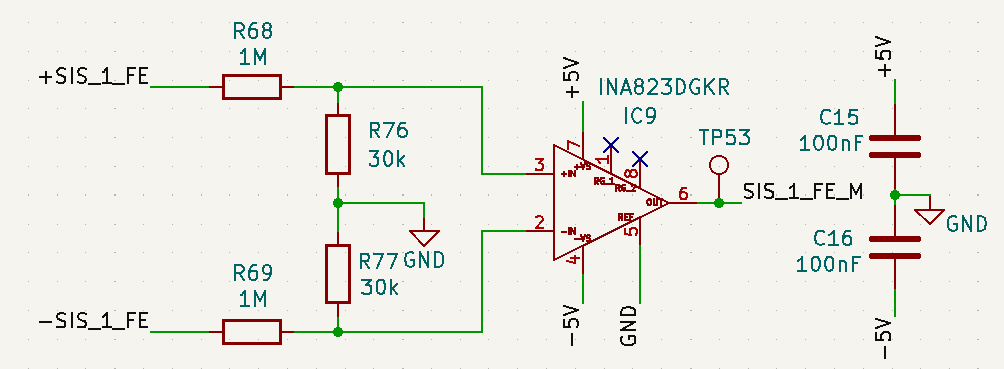
\includegraphics[width = \linewidth]{img/sis_medicion.png}
    \caption{Esquemático del circuito de medición de los SIS}
    \label{fig:sis_medicion}
\end{figure}


